\subsection{Server Recovery}
\label{sub:eval:server-recovery}

We define server recovery as the amount of time it takes for \APIName to publish a new server after a server failure.
In order to compute recovery time, we measured events related to devices disconnection and server publication, as presented
in Listing~\ref{lst:events:server-recovery}. 


Figure~\ref{fig:server-recovery} presents the cumulative empirical function for server recovery time.
In most of the cases, server recovery happens under 15 seconds. 
However, in some corner cases scenarios, it took almost 1 minute for server recovery. 
It is worth noting that this recovery time takes into account the DNS-SD service discovery time, 
i.e. the time it takes for the service discovery protocol to detect that the last running service with a given name is not available anymore until a new server is published with the same name. 



\begin{figure}
    \centering
    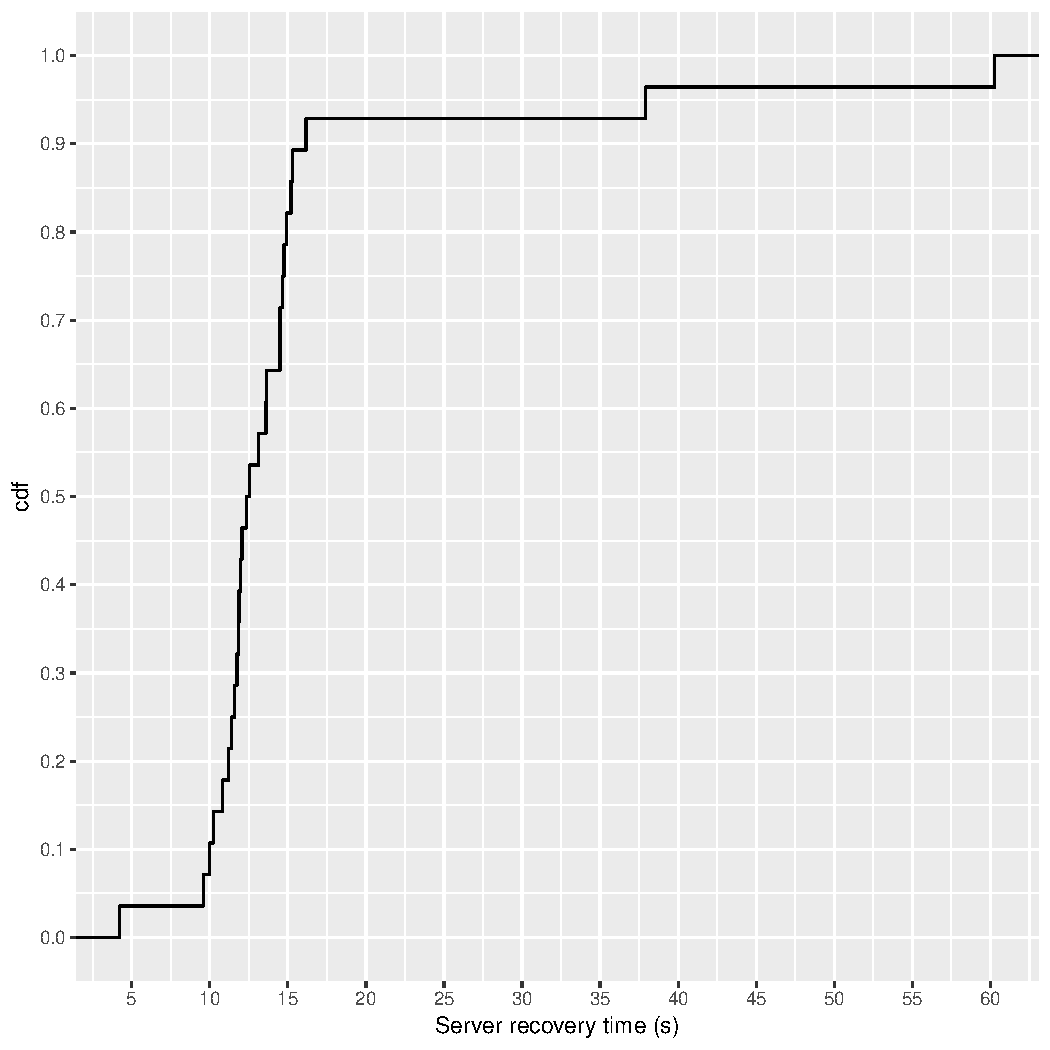
\includegraphics[width=0.9\linewidth]{server-recovery}
    \caption{Server Recovery Time}
    \label{fig:server-recovery}
\end{figure}


Despite recovering under 15 seconds in most of the cases,
we acknowledge that our current recovery time uncovers some flaws of our API stack.
For instance, while the server died but before clients detected that, several operations could have been called and these operations would have to be re-executed once a new server was discovered, 
or in longer scenarios, users may question if~\APIName is the right approach to build local browser applications and they may consider alternative solutions.
We believe that our measured values could be improved and server recovery should be faster if we tackle some critical bottlenecks of our API stack.
As an example, one could use more a aggressive protocol for service discovery~\cite{hong2007accelerating}, 
thus diminishing discovery time, or the first successor could have a running background server since startup.
As soon as this successor detected a failure, it could publish its background server, 
hence server startup time would be diminished as well. 
